\section{Aufbau}
\label{sec:Aufbau}

Der Aufbau besteht aus einem Helium-Neon-Laser mit einer Wellenlänge von $\lambda = \SI{635}{\nano\metre}$. Dieser trifft senkrecht auf einen Einzel- beziehungsweise Doppelspalt, sodass das Licht nach Fraunhofer Art gebeugt wird. In einem Abstand von $L=\SI{1}{\metre}$ befindet sich ein Photoelement auf einem Verschiebereiter, mit dem mittels eines Amperemeters die Lichtintensität zur Bestimmung der Beugungsfigur gemessen werden kann.

\begin{figure}
	\centering
	\caption{Skizze des Versuchsaufbaus zur Messung der Beugungsfiguren \cite{V406}.}
	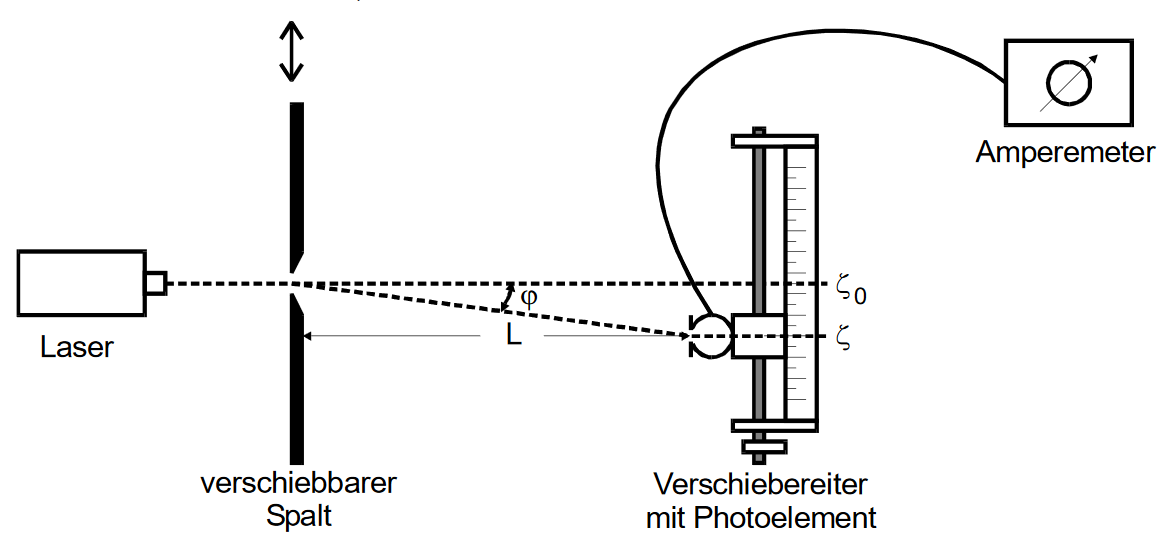
\includegraphics[width=\linewidth-70pt,height=\textheight-70pt,keepaspectratio]{content/images/Aufbau.png}
	\label{fig:Aufbau}
\end{figure}